

\begin{chapter}{Funciones de Prueba}

\section{Comparativa ZDT (Zitzler-Deb-Thiele)} 

\subsection*{ZDT1}

Tiene un {\it frente de Pareto} convexo:\\

\begin{align*}
f_1(x)=x_1\\
f_2(x,g)=g(x)(1-\sqrt{ \frac{f_1}{g(x)}})\\
g(x)=1+\frac{9}{n-1}\sum_{i=2}^nx_i
\end{align*}

donde $n=30$, y $x_i\in[0,1]$. El $F_\text{verdadero}$ es formado con $g(x)=1$ y es mostrado en la figura \ref{fig:ZDT1}.

\begin{figure}[h!]
 \centering
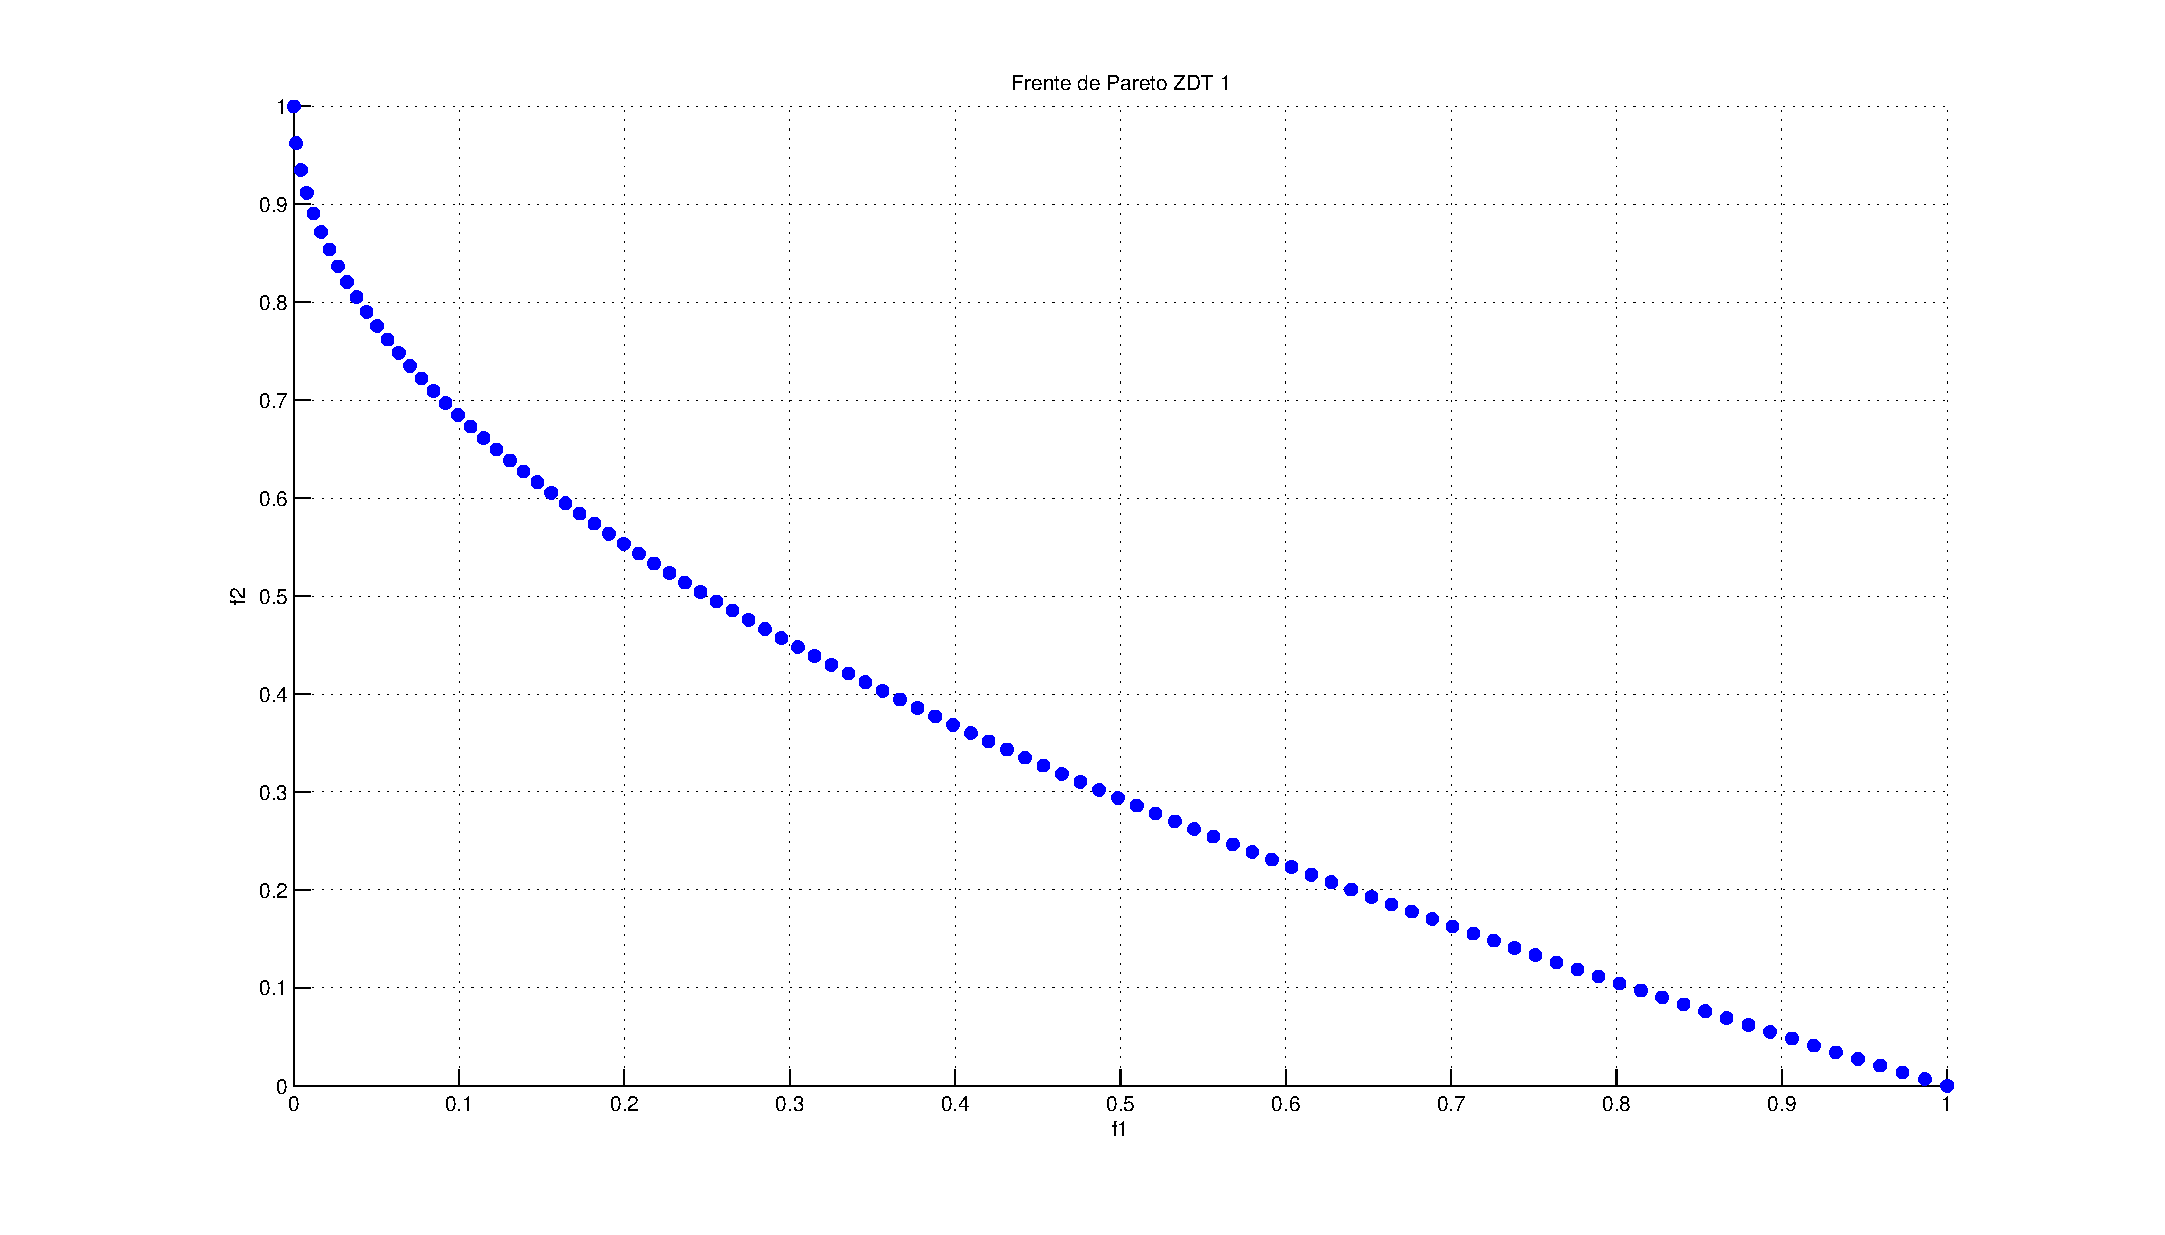
\includegraphics[width=200pt]{Apendices/paretoZDT1.eps}
\caption{Frente de Pareto ZDT1}
\label{fig:ZDT1}
\end{figure} 

\subsection*{ZDT2}

Tiene un {\it frente de Pareto} c\'oncavo:\\

\begin{align*}
f_1(x)&=x_1\\
f_2(x,g)&=g(x)(1-( \frac{f_1}{g(x)})^2)\\
g(x)&=1+\frac{9}{n-1}\sum_{i=2}^nx_i
\end{align*}

donde $n=30$, y $x_i\in[0,1]$. El $F_\text{verdadero}$ es formado con $g(x)=1$ y es mostrado en la figura \ref{fig:ZDT2}..


\begin{figure}[h!]
 \centering
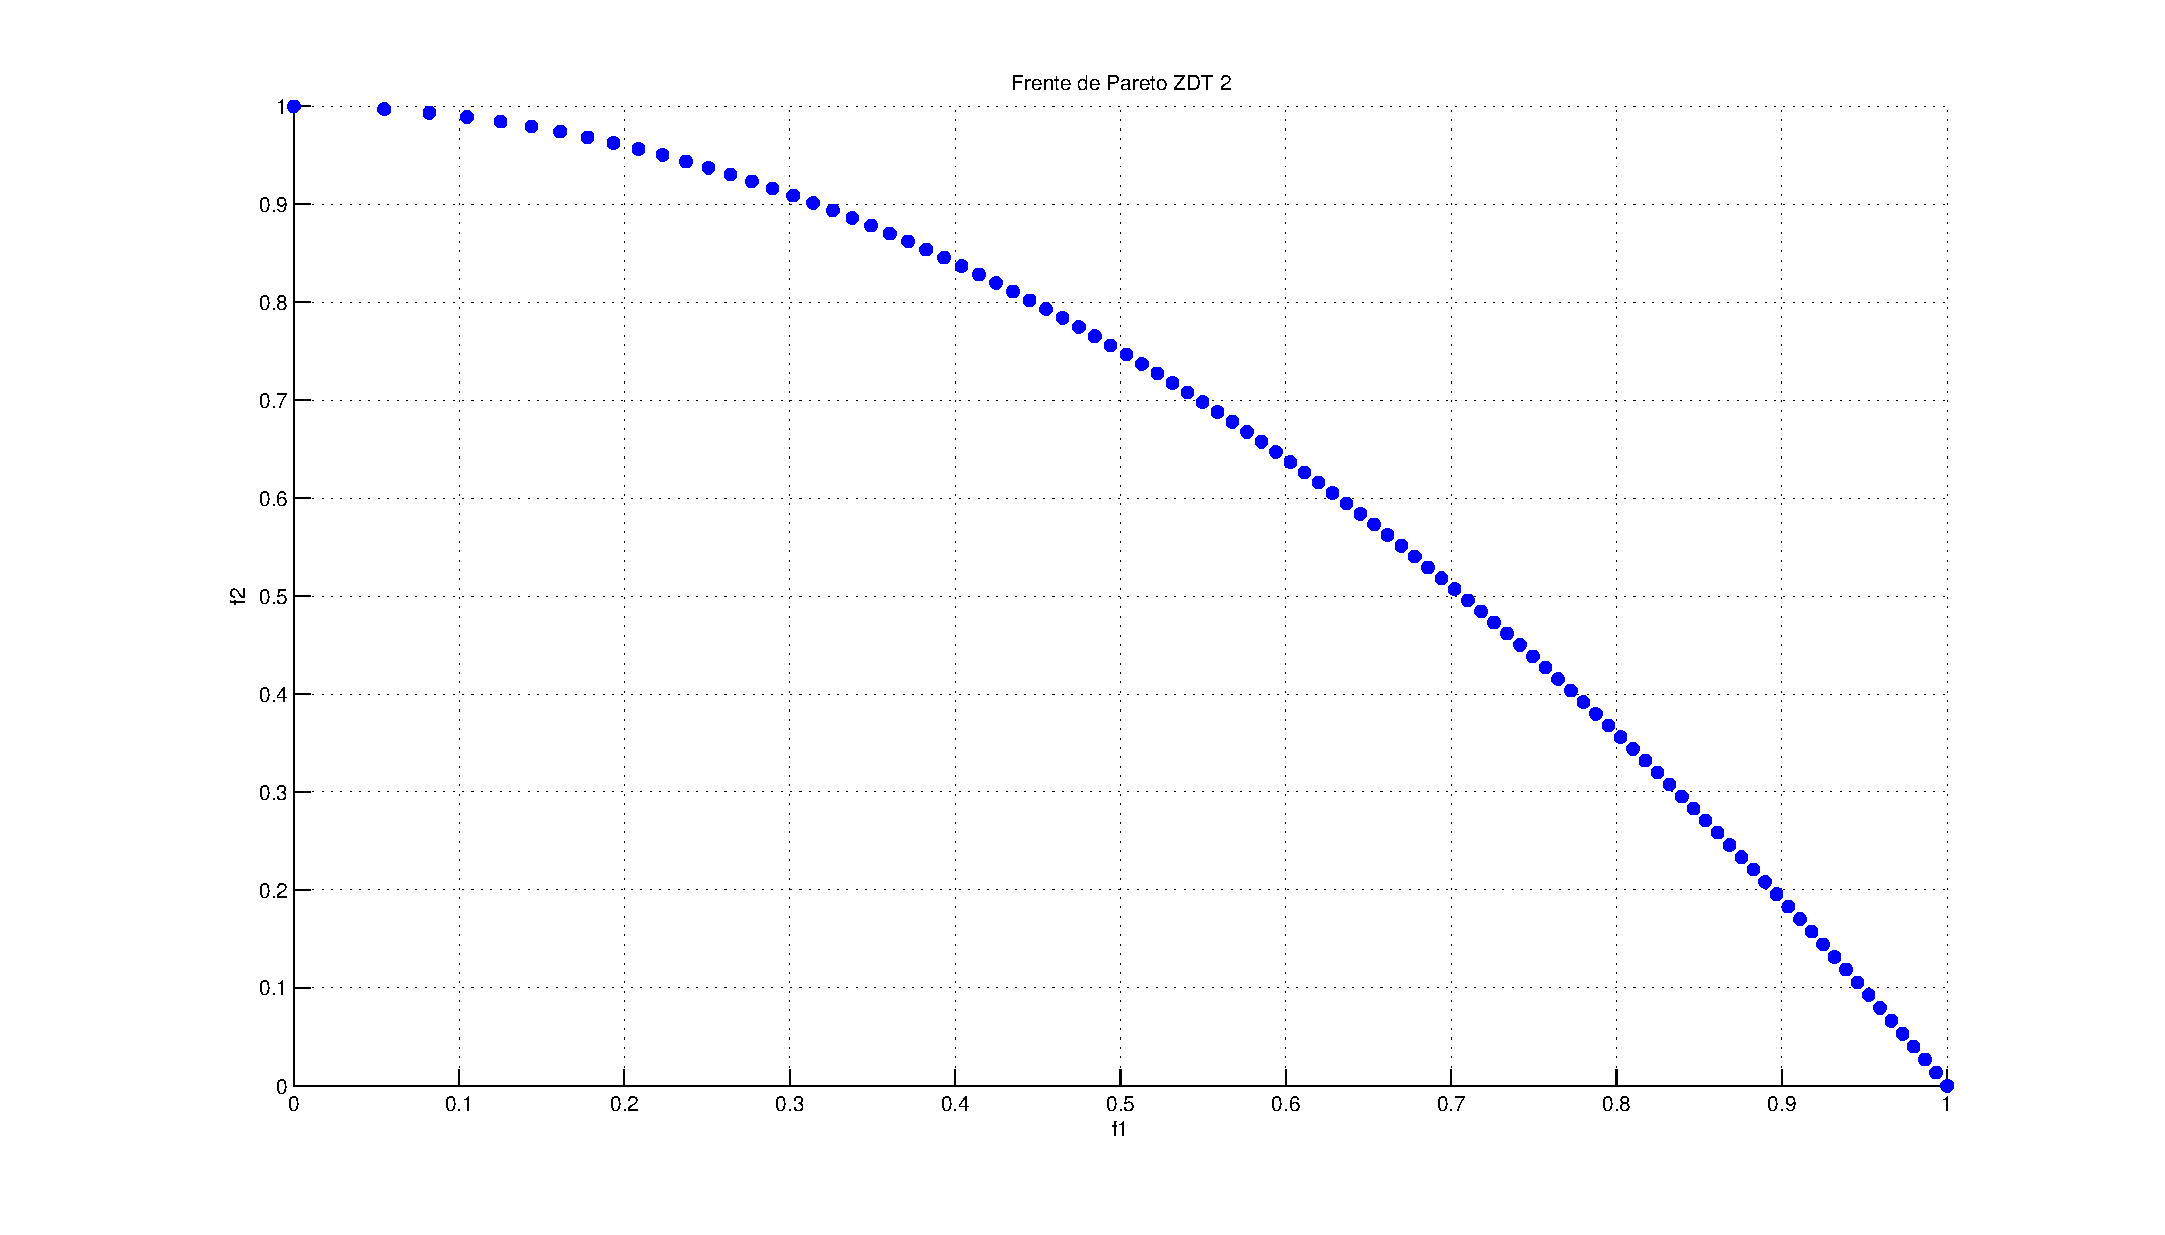
\includegraphics[width=200pt]{Apendices/paretoZDT2.eps}
\caption{Frente de Pareto ZDT2}
\label{fig:ZDT2}
\end{figure} 

\subsection*{ZDT3}

Tiene un {\it frente de Pareto}  discontinuo, convexo:\\

\begin{align*}
f_1(x)&=x_1,\\
f_2(x,g)&=g(x)(1-\sqrt{\frac{f_1}{g(x)}}-\frac{f_1}{g(x)}\sin(10\pi f_1))\\
g(x)&=1+\frac{9}{n-1}\sum_{i=2}^nx_i
\end{align*}

donde $n=30$, y $x_i\in[0,1]$. El $F_\text{verdadero}$ es formado con $g(x)=1$ y es mostrado en la figura \ref{fig:ZDT3}..




\begin{figure}[h!]
 \centering
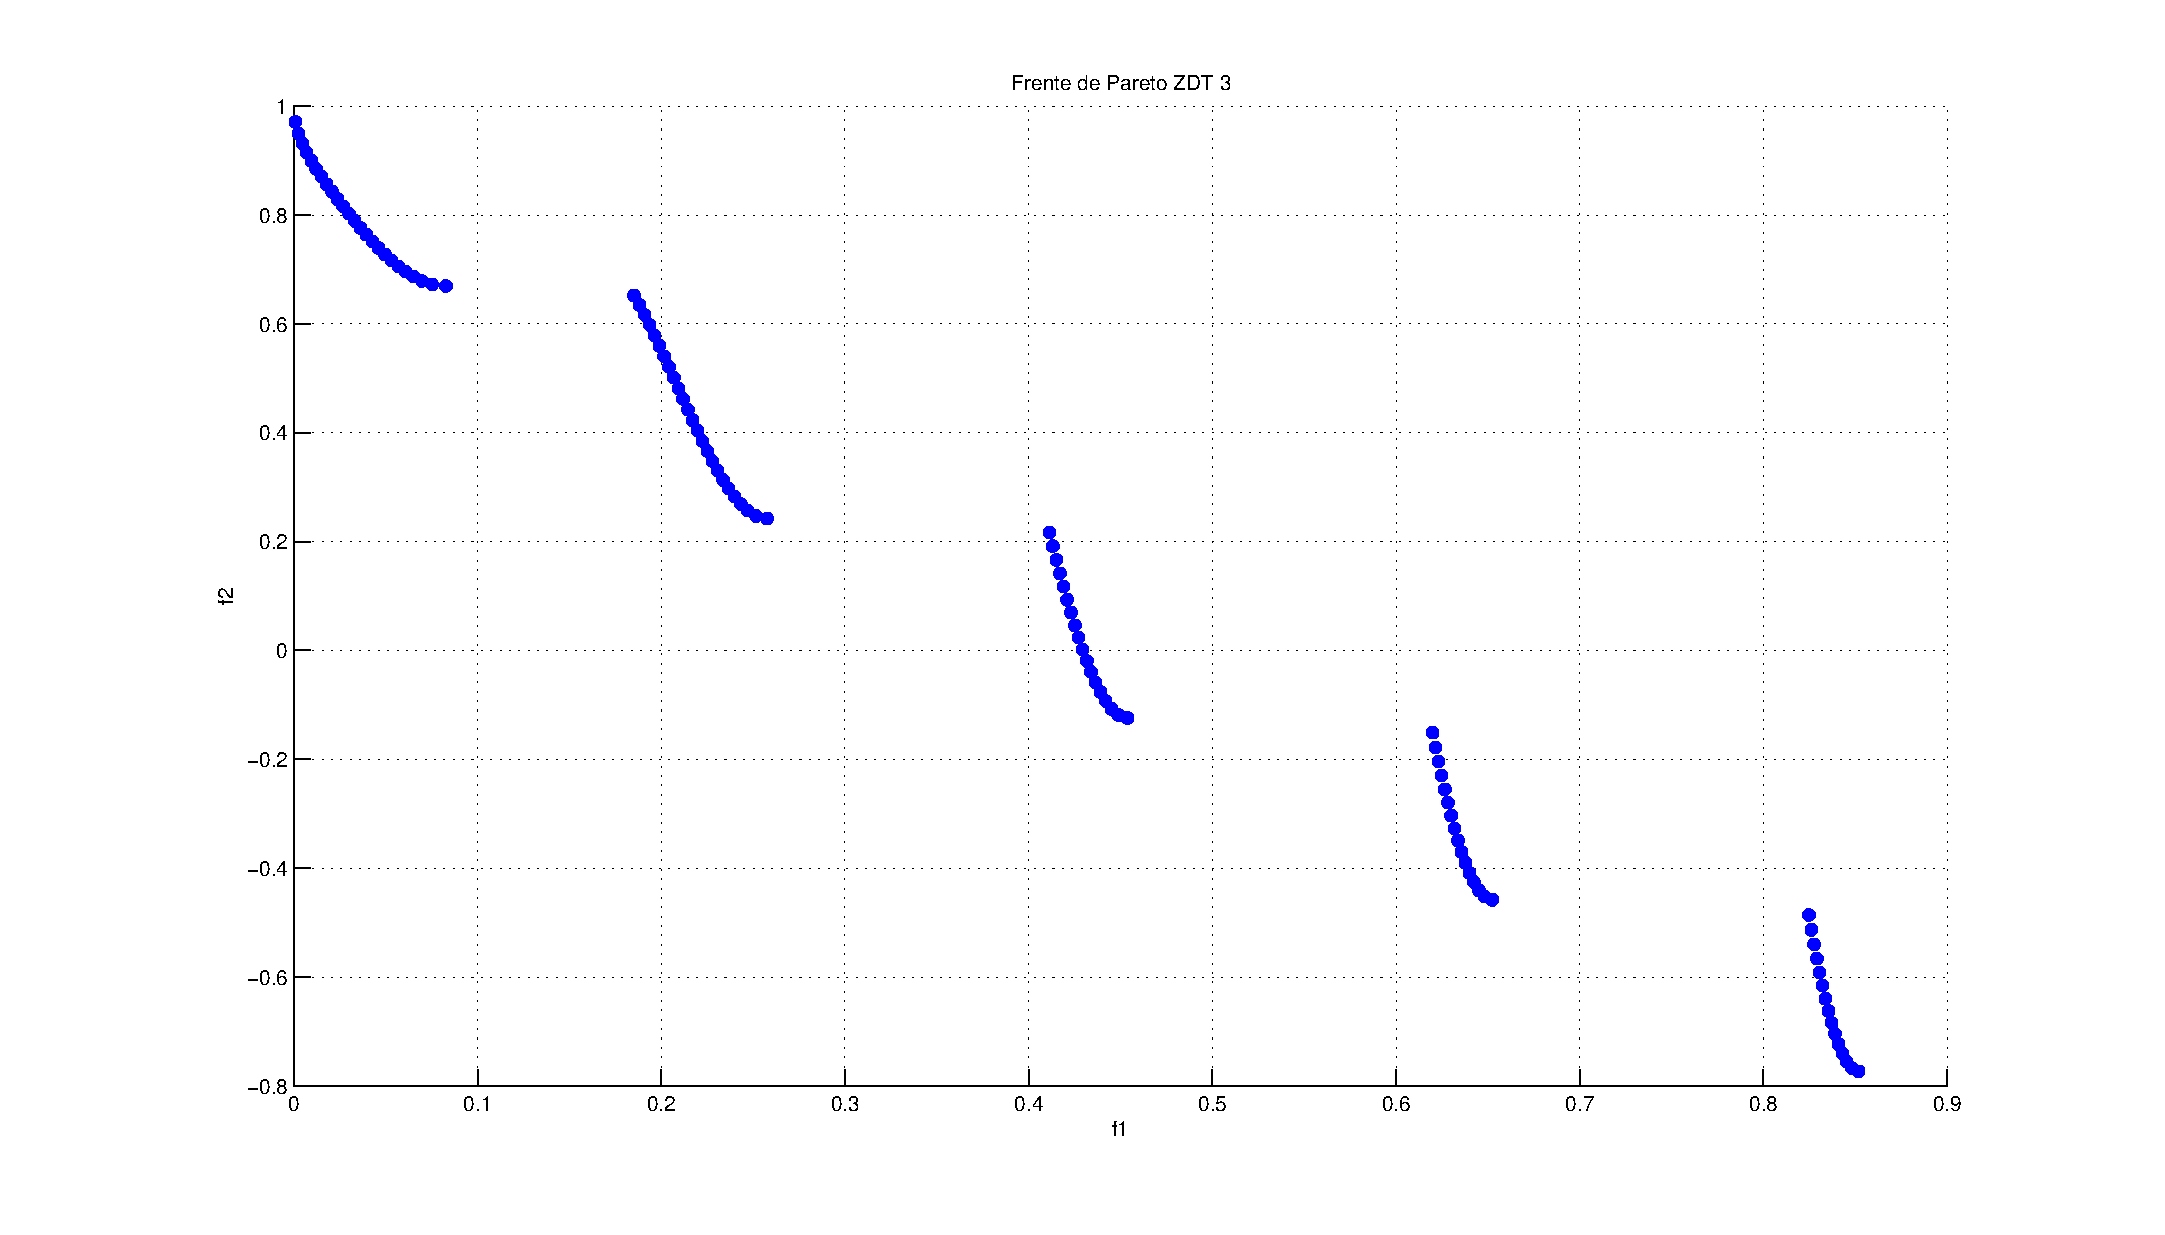
\includegraphics[width=200pt]{Apendices/paretoZDT3.eps}
\caption{Frente de Pareto ZDT3}
\label{fig:ZDT3}
\end{figure} 






\subsection*{ZDT4}

Tiene  $21^9$ frentes locales, lo que pone a prueba la habilidad de los AEMOs de lidiar con problemas multifrontales:\\

\begin{align*}
f_1(x)&=x_1,\\
f_2(x,g)&=g(x)(1-\sqrt{ \frac{f_1}{g(x)}}),\\
g(x)&=1+10 (n-1)+ \sum_{i=2}^n(x_i^2-10cos(4\pi x_i))
\end{align*}

donde $n=10$, y $x_1\in[0,1]$ y $x_2,...x_n\in[-5,5]$. El $F_\text{verdadero}$ es formado con $g(x)=1$ y es mostrado en la figura \ref{fig:ZDT4}.

\begin{figure}[h!]
 \centering
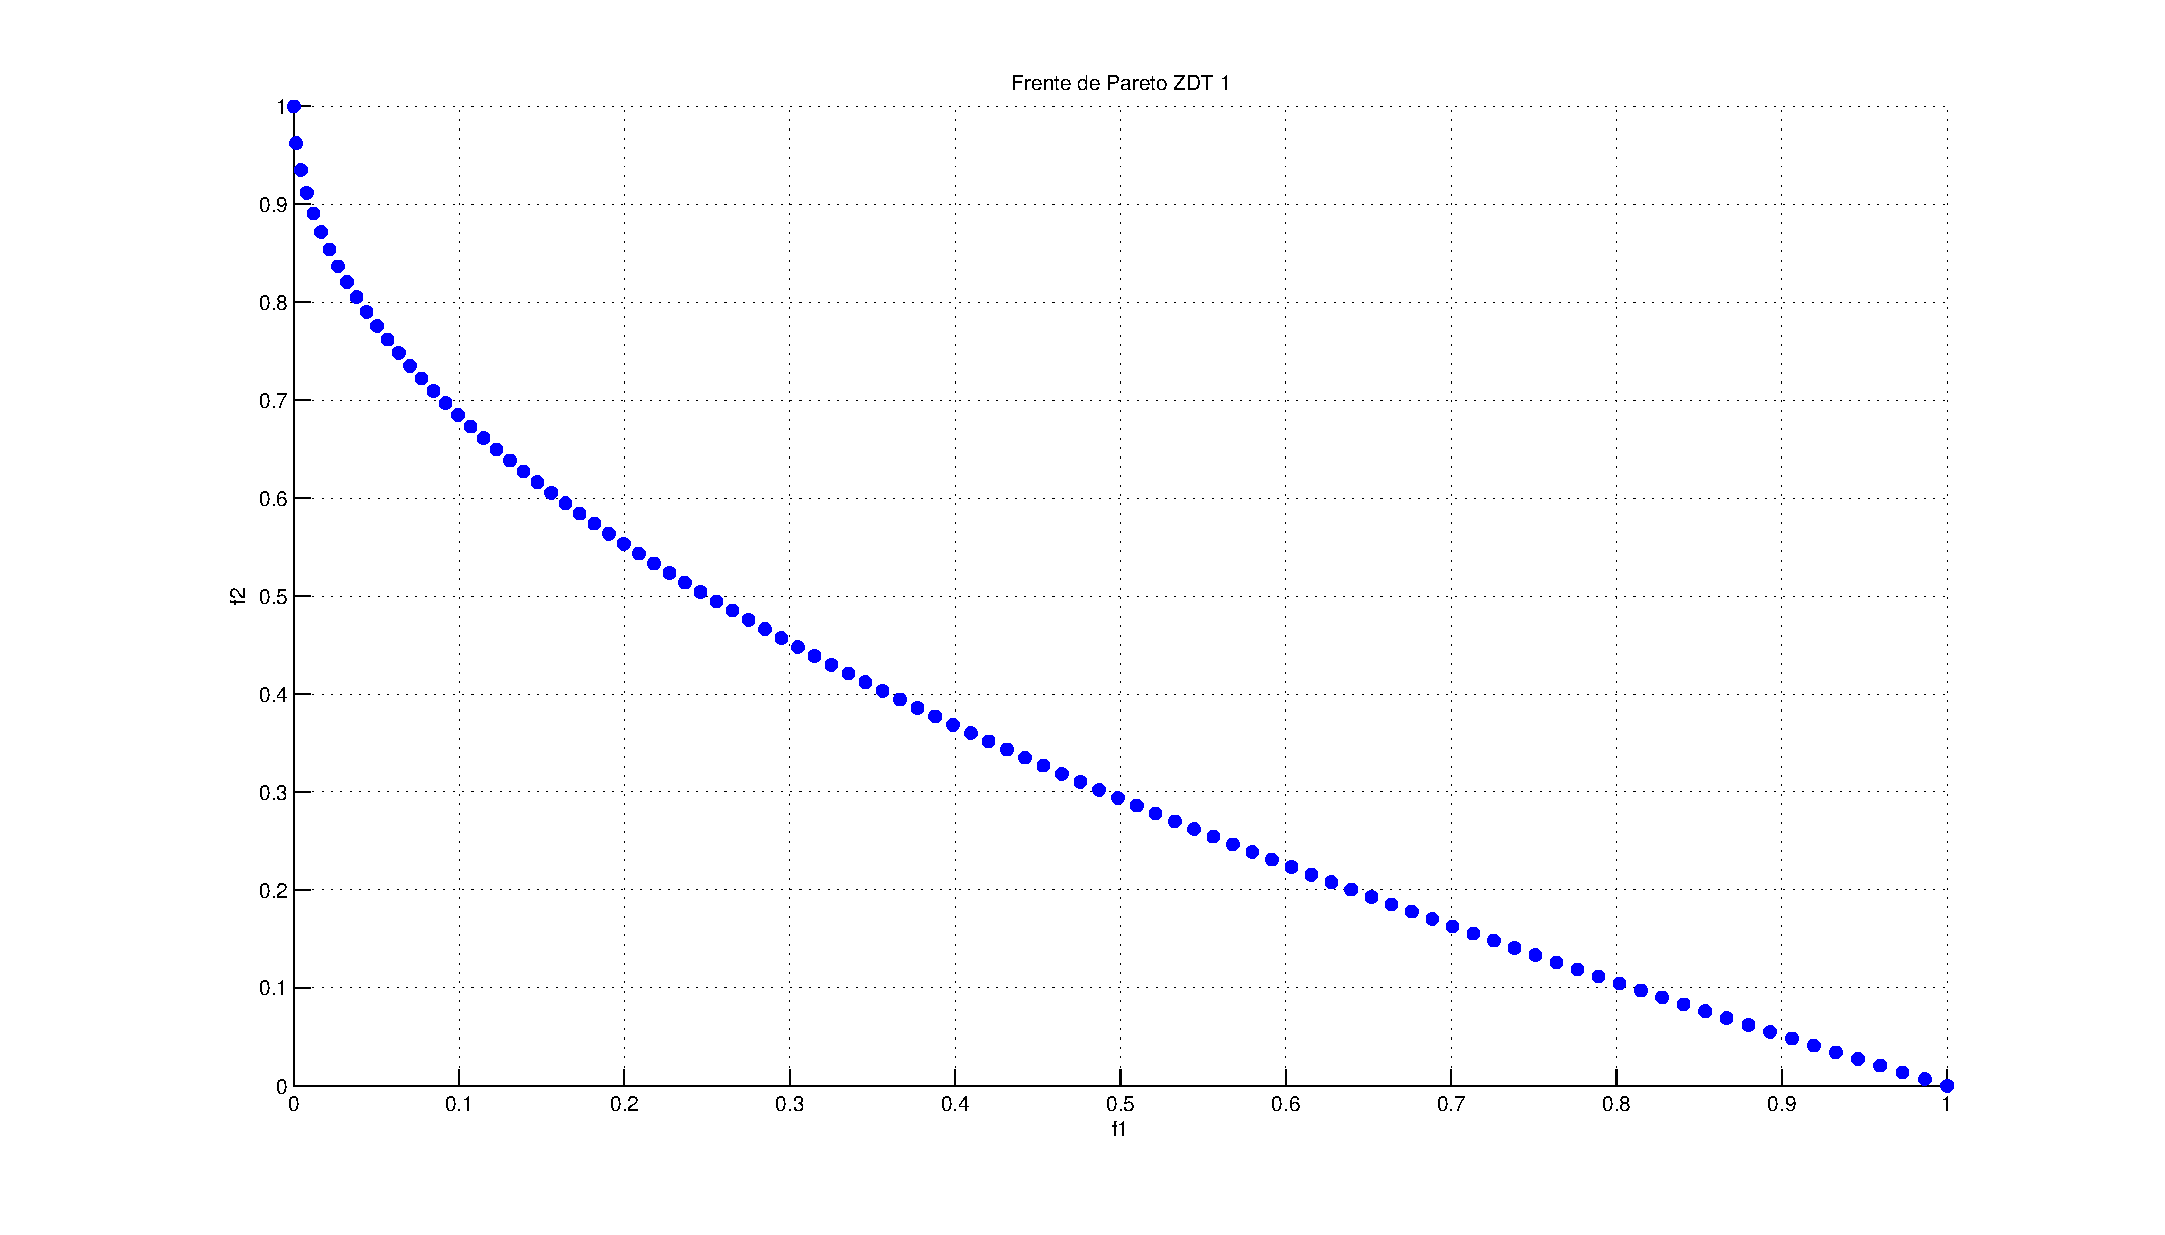
\includegraphics[width=200pt]{Apendices/paretoZDT1.eps}
\caption{Frente de Pareto ZDT4}
\label{fig:ZDT4}
\end{figure} 


\subsection*{ZDT6}



El espacio de b\'usqueda en este problema es no uniforme, la densidad de las soluciones es baja cerca del $F_{\text {verdadero}}$ y alta lejos del frente.



\begin{align*}
f_1(x)&=1-exp(-4x_1)\sin^6(6\pi x_1),\\
f_2(x,g)&=g(x)(1-(\frac{f_1}{g(x)})^2),\\
g(x)&=1+9[\frac{\sum_{i=2}^n}{9}]^{0.25}
\end{align*}



donde $n=10$, y $x_1\in[0,1]$ y $x_2,...x_n\in[-5,5]$. El $F_\text{verdadero}$ es formado con $g(x)=1$ y es mostrado en la figura \ref{fig:ZDT6}.

\begin{figure}[h!]
 \centering
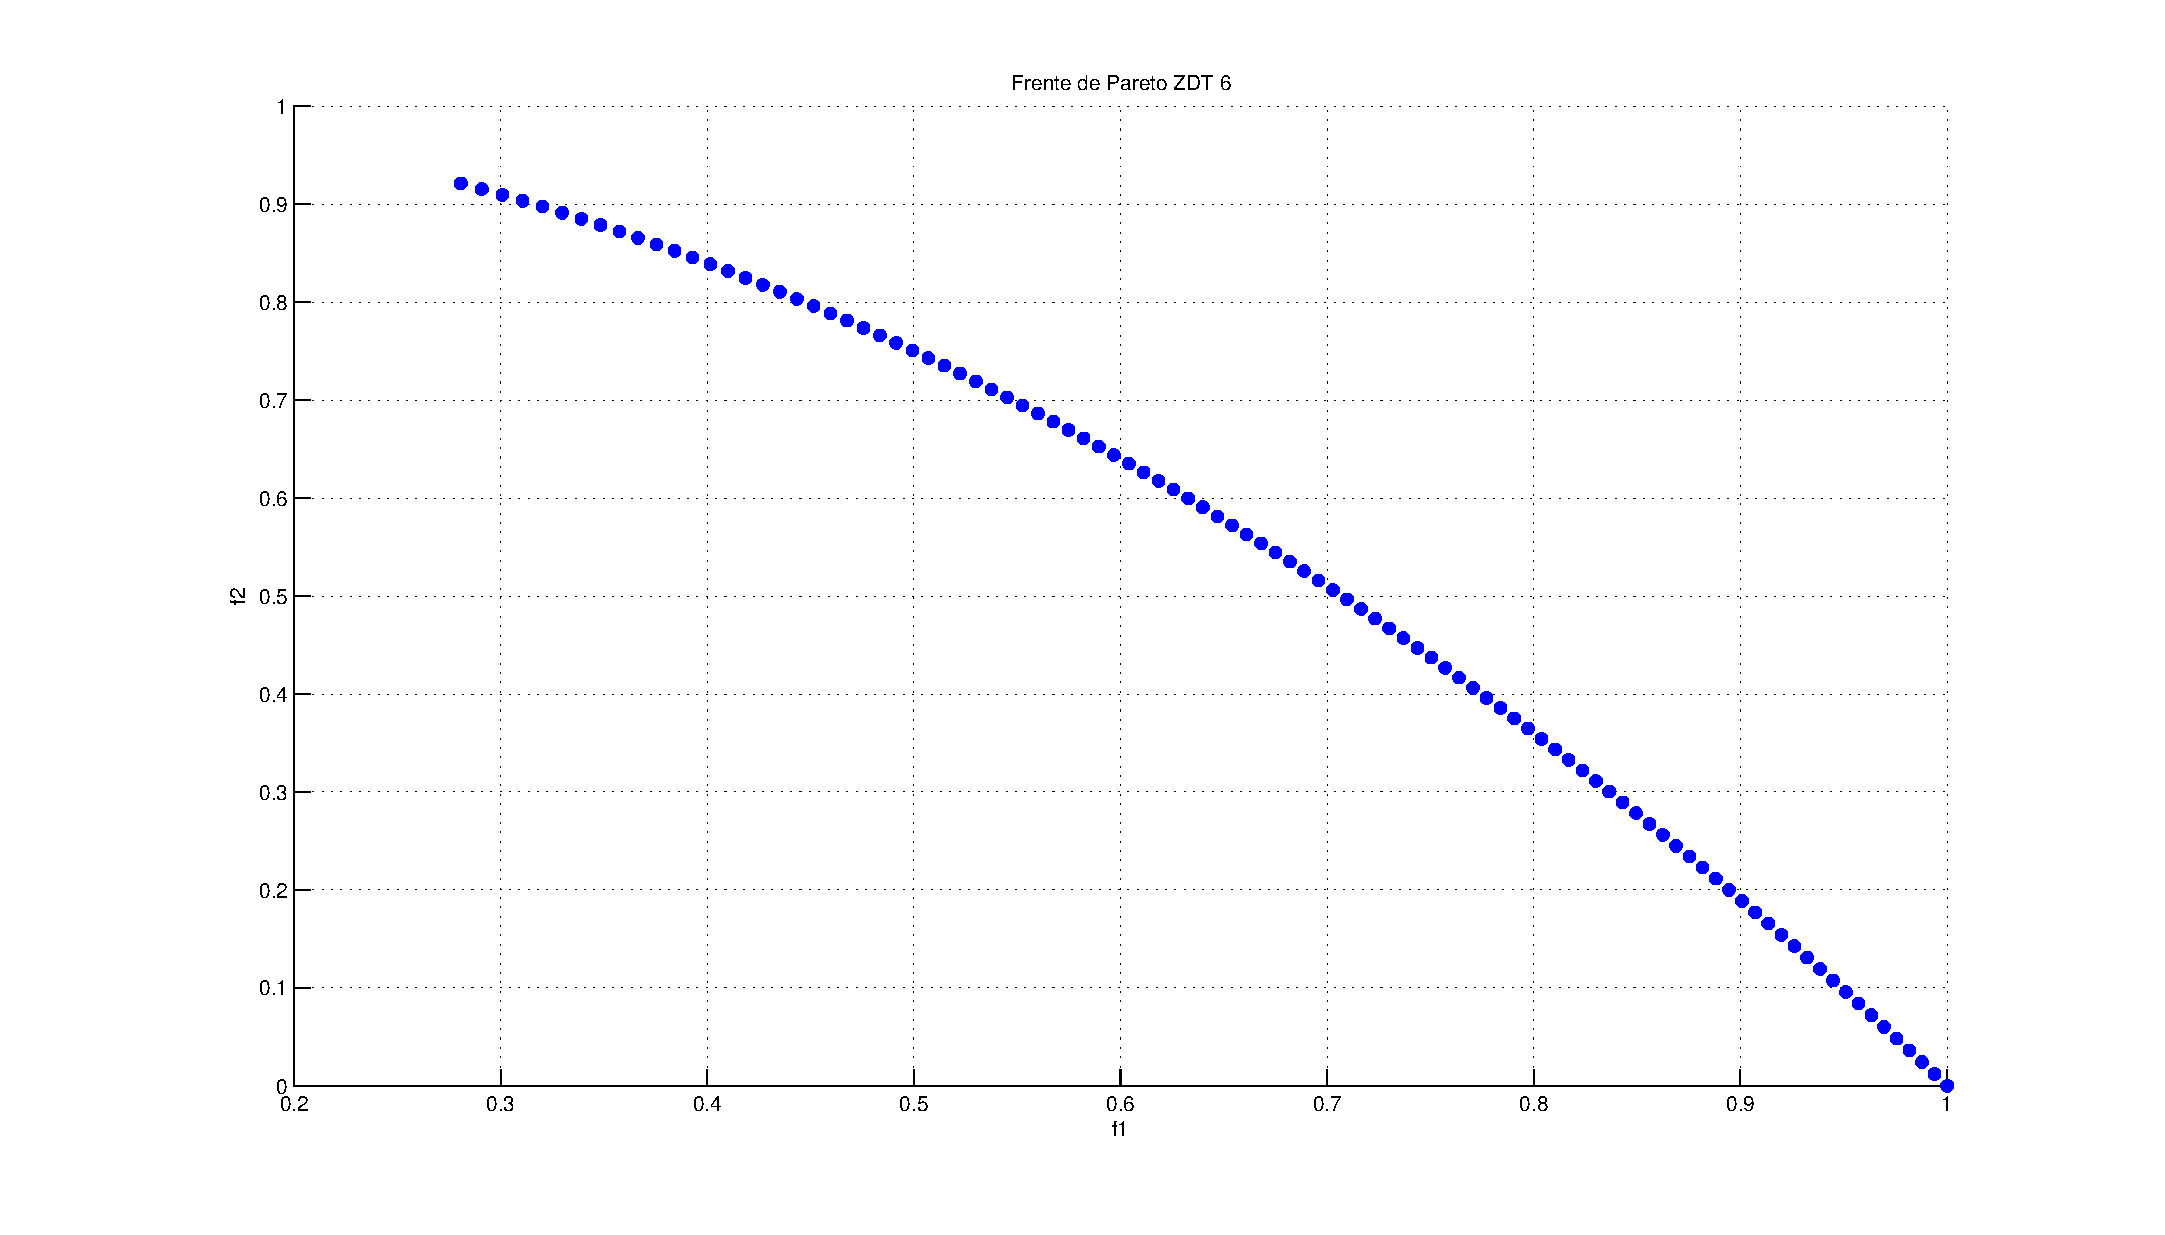
\includegraphics[width=200pt]{Apendices/paretoZDT6.eps}
\caption{Frente de Pareto ZDT6}
\label{fig:ZDT6}
\end{figure} 



\section{Comparativa DTLZ (Deb-Thiele-Laumanns-Zitzler)} 


\subsection*{DTLZ1}


Tiene un {\it frente de Pareto}  lineal, separable, multimodal.\\


\begin{align*}
f_1(x)&=\frac{1}{2}x_1x_2\hdots x_{M-1}(1+g(x))\\
f_2(x)&=\frac{1}{2}x_1x_2\hdots (1-x_{M-1})(1+g(x))\\
\vdots&\\
f_M(x)&=\frac{1}{2}(1-x_1)(1+g(x))\\
g(x)&=100[k+\sum_{i=M}^n(x_i-0.5)^2-cos(20\pi(x_i-0.5))]
\end{align*}


donde $n=M+k-1$ (un valor de $k=5$ es sugerido) y $x_i\in[0,1]$. El espacio de
b\'usqueda contiene $11^k-1$ frentes locales. El $F_\text{verdadero}$ para $M=3$ es mostrado en la figura \ref{fig:DTLZ1}. 

\begin{figure}[h!]
 \centering
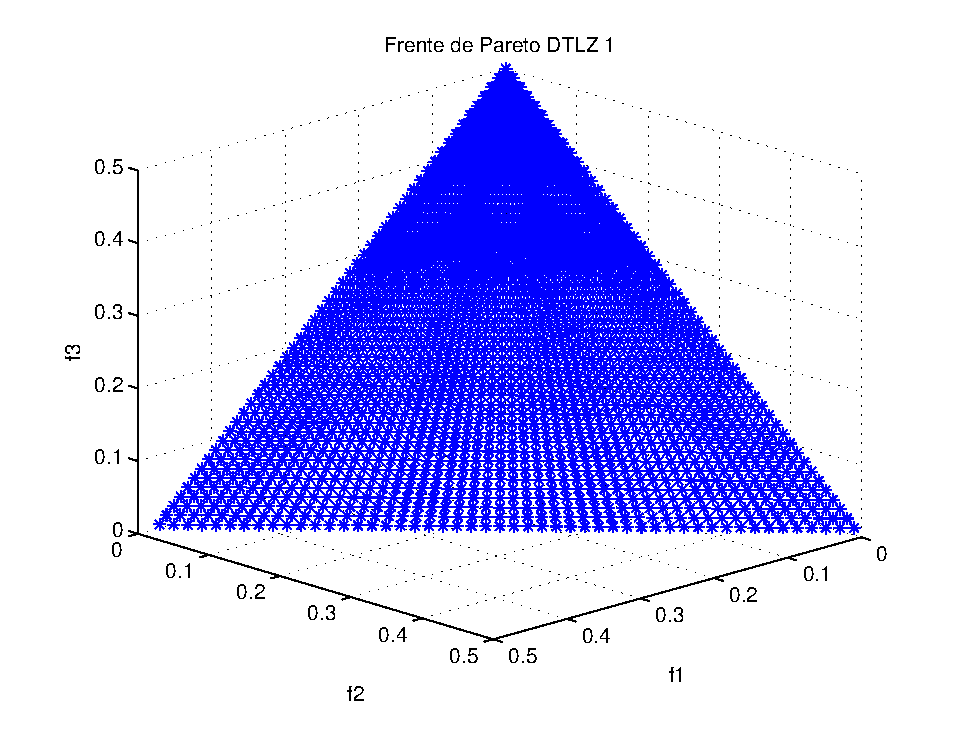
\includegraphics[width=200pt]{Apendices/paretoDTLZ1.eps}
\caption{Frente de Pareto DTLZ1}
\label{fig:DTLZ1}
\end{figure}



\subsection*{DTLZ2}


Tiene un {\it frente de Pareto}  c\'oncavo. Esta funci\'on puede ser usada para investigar la habilidad de un AEMO de escalar su rendimiento a 
muchos objetivos.\\


\begin{align*}
f_1(x)&=cos(x_1\frac{\pi}{2})cos(x_2\frac{\pi}{2})\hdots cos(x_{M-1}\frac{\pi}{2})(1+g(x))\\
f_2(x)&=cos(x_1\frac{\pi}{2})cos(x_2\frac{\pi}{2})\hdots sin(x_{M-1}\frac{\pi}{2})(1+g(x))\\
f_3(x)&=cos(x_1\frac{\pi}{2})cos(x_2\frac{\pi}{2})\hdots sin(x_{M-2}\frac{\pi}{2})(1+g(x))\\
\vdots&\\
f_{M-1}(x)&=cos(x_1\frac{\pi}{2})sin(x_2\frac{\pi}{2})(1+g(x))\\
f_{M}(x)&=sin(x_1\frac{\pi}{2})(1+g(x))\\
g(x)&=\sum_i=(x_i-0.5)^2
\end{align*}


donde $n=M+k-1$ (un valor de $k=10$ es sugerido) y $x_i\in[0,1]$. El $F_\text{verdadero}$ para $M=3$ es mostrado en la figura \ref{fig:DTLZ2}. 

\begin{figure}[h!]
 \centering
\includegraphics[width=200pt]{Apendices/paretoDTLZ2.eps}
\caption{Frente de Pareto DTLZ2}
\label{fig:DTLZ2}
\end{figure}



\subsection*{DTLZ3}

Es el mismo que DTLZ2 excepto por una nueva funci\'on $g(x)$. Tiene un {\it frente de Pareto}  c\'oncavo, multimodal. Prueba la habilidad de un AEMO de converger al $F_\text{verdadero}$.\\



\begin{align*}
f_1(x)&=cos(x_1\frac{\pi}{2})cos(x_2\frac{\pi}{2})\hdots cos(x_{M-1}\frac{\pi}{2})(1+g(x))\\
f_2(x)&=cos(x_1\frac{\pi}{2})cos(x_2\frac{\pi}{2})\hdots sin(x_{M-1}\frac{\pi}{2})(1+g(x))\\
f_3(x)&=cos(x_1\frac{\pi}{2})cos(x_2\frac{\pi}{2})\hdots sin(x_{M-2}\frac{\pi}{2})(1+g(x))\\
\vdots&\\
f_{M-1}(x)&=cos(x_1\frac{\pi}{2})sin(x_2\frac{\pi}{2})(1+g(x))\\
f_{M}(x)&=sin(x_1\frac{\pi}{2})(1+g(x))\\
g(x)&=100[k+\sum_{i=M}^n(x_i-0.5)^2-cos(20\pi(x_i-0.5))]
\end{align*}


donde $n=M+k-1$ (un valor de $k=10$ es sugerido) y $x_i\in[0,1]$. La  funci\'on $g(x)$ introduce  $3k-1$ frentes locales paralelos al frente global.
El $F_\text{verdadero}$ para $M=3$ es mostrado en la figura \ref{fig:DTLZ3}. 

\begin{figure}[h!]
 \centering
\includegraphics[width=200pt]{Apendices/paretoDTLZ2.eps}
\caption{Frente de Pareto DTLZ3}
\label{fig:DTLZ3}
\end{figure}




\subsection*{DTLZ4}


Tiene un {\it frente de Pareto}  c\'oncavo, separable, multimodal. Esta funci\'on prueba la habilidad
de los AEMOs de mantener una buena distribuci\'on de las soluciones.


\begin{align*}
f_1(x)&=cos(x_1^\alpha\frac{\pi}{2})cos(x_2^\alpha\frac{\pi}{2})\hdots cos(x_{M-1}^\alpha\frac{\pi}{2})(1+g(x))\\
f_2(x)&=cos(x_1^\alpha\frac{\pi}{2})cos(x_2^\alpha\frac{\pi}{2})\hdots sin(x_{M-1}^\alpha\frac{\pi}{2})(1+g(x))\\
f_3(x)&=cos(x_1^\alpha\frac{\pi}{2})cos(x_2^\alpha\frac{\pi}{2})\hdots sin(x_{M-2}^\alpha\frac{\pi}{2})(1+g(x))\\
\vdots&\\
f_{M-1}(x)&=cos(x_1^\alpha\frac{\pi}{2})sin(x_2^\alpha\frac{\pi}{2})(1+g(x))\\
f_{M}(x)&=sin(x_1^\alpha\frac{\pi}{2})(1+g(x))\\
g(x)&=\sum_i=(x_i-0.5)^2
\end{align*}


donde $n=M+k-1$ ($k=10$ y $\alpha=100$ son sugeridos) y $x_i\in[0,1]$. El $F_\text{verdadero}$ para $M=3$ es mostrado en la figura \ref{fig:DTLZ4}. 

\begin{figure}[h!]
 \centering
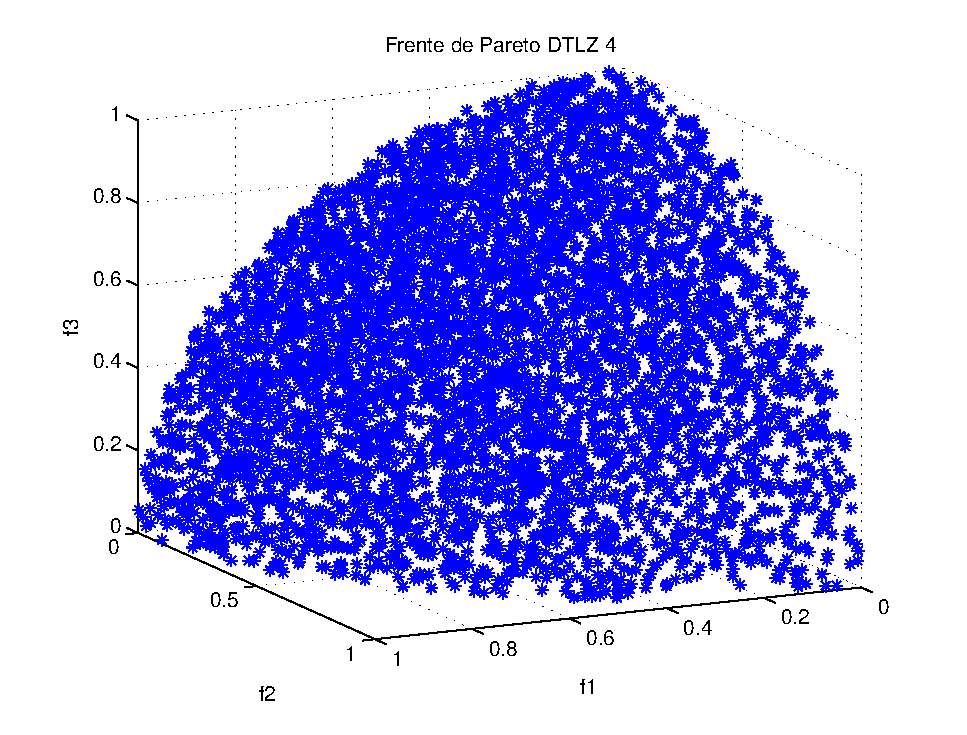
\includegraphics[width=200pt]{Apendices/paretoDTLZ4.eps}
\caption{Frente de Pareto DTLZ4}
\label{fig:DTLZ4}
\end{figure}




\subsection*{DTLZ25}


Tiene un {\it frente de Pareto}  curvo.\\


\begin{align*}
f_1(x)&=cos(\theta_1\frac{\pi}{2})cos(\theta_2\frac{\pi}{2})\hdots cos(\theta_{M-1}\frac{\pi}{2})(1+g(x))\\
f_2(x)&=cos(\theta_1\frac{\pi}{2})cos(\theta_2\frac{\pi}{2})\hdots sin(\theta_{M-1}\frac{\pi}{2})(1+g(x))\\
f_3(x)&=cos(\theta_1\frac{\pi}{2})cos(\theta_2\frac{\pi}{2})\hdots sin(\theta_{M-2}\frac{\pi}{2})(1+g(x))\\
\vdots&\\
f_{M-1}(x)&=cos(\theta_1\frac{\pi}{2})sin(\theta_2\frac{\pi}{2})(1+g(x))\\
f_{M}(x)&=sin(\theta_1\frac{\pi}{2})(1+g(x))\\
\theta_1&=\frac{\pi}{2}x_1\\
\theta_i&=\frac{\pi}{4(1+g(x))}(1+2g(x)x_i),  &\text{para} i=2,3\dots,(M-1)\\
g(x)&=\sum_i=(x_i-0.5)^2
\end{align*}


donde $n=M+k-1$ (un valor de $k=10$ es sugerido) y $x_i\in[0,1]$. El $F_\text{verdadero}$ para $M=3$ es mostrado en la figura \ref{fig:DTLZ5}. 

\begin{figure}[h!]
 \centering
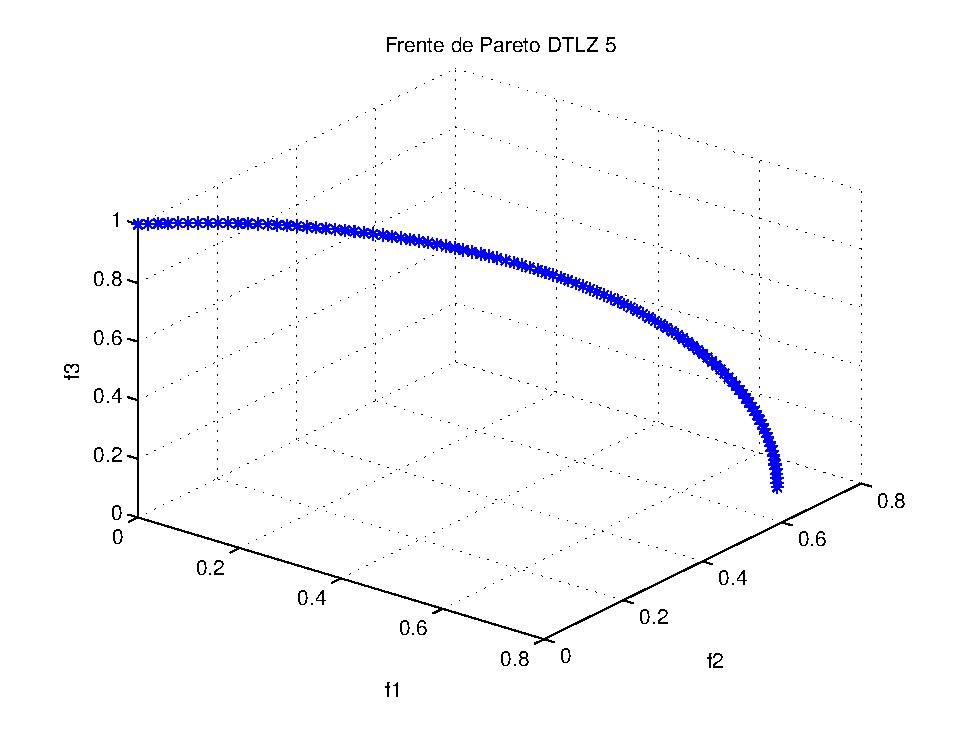
\includegraphics[width=200pt]{Apendices/paretoDTLZ5.eps}
\caption{Frente de Pareto DTLZ5}
\label{fig:DTLZ5}
\end{figure}




\subsection*{DTLZ6}


Modifica la funci\'on $g(x)$ de DTLZ5 volvi\'endolo un problema m\'as dif\'icil. Tiene un {\it frente de Pareto}  curvo.\\


\begin{align*}
f_1(x)&=cos(\theta_1\frac{\pi}{2})cos(\theta_2\frac{\pi}{2})\hdots cos(\theta_{M-1}\frac{\pi}{2})(1+g(x))\\
f_2(x)&=cos(\theta_1\frac{\pi}{2})cos(\theta_2\frac{\pi}{2})\hdots sin(\theta_{M-1}\frac{\pi}{2})(1+g(x))\\
f_3(x)&=cos(\theta_1\frac{\pi}{2})cos(\theta_2\frac{\pi}{2})\hdots sin(\theta_{M-2}\frac{\pi}{2})(1+g(x))\\
\vdots&\\
f_{M-1}(x)&=cos(\theta_1\frac{\pi}{2})sin(\theta_2\frac{\pi}{2})(1+g(x))\\
f_{M}(x)&=sin(\theta_1\frac{\pi}{2})(1+g(x))\\
\theta_1&=\frac{\pi}{2}x_1\\
\theta_i&=\frac{\pi}{4(1+g(x))}(1+2g(x)x_i)  &\text{para } i=2,3\dots,(M-1)\\
g(x)&=\sum_i=(x_i-0.5)^0.1
\end{align*}


donde $n=M+k-1$ (un valor de $k=10$ es sugerido) y $x_i\in[0,1]$. El $F_\text{verdadero}$ para $M=3$ es mostrado en la figura \ref{fig:DTLZ6}. 

\begin{figure}[h!]
 \centering
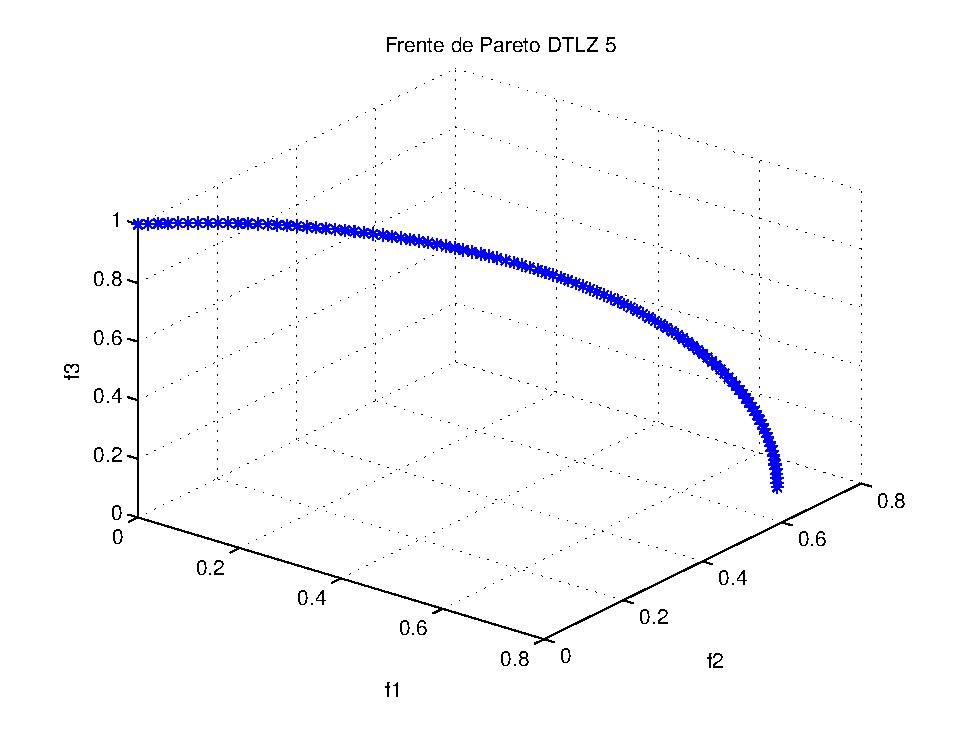
\includegraphics[width=200pt]{Apendices/paretoDTLZ5.eps}
\caption{Frente de Pareto DTLZ6}
\label{fig:DTLZ6}
\end{figure}



\subsection*{DTLZ7}

Tiene un {\it frente de Pareto}  discontinuo. Este problema prueba la habilidad de un AEMO de mantener
individuos en las diferentes regiones del {\it frente de Pareto}.\\


\begin{align*}
f_1(x)&=x_1
f_2(x)&=x_2\\
\vdots&\\
f_{M-1}(x)&=x_{M-1}\\
f_{M}(x)&=(1+g(x_M))h(f_1,f_2,\dots,f_{M-1}g(x))\\
g(x)&=1+\frac{9}{k}\sum_{i=2}^nx_i\\
h(f_1,f_2,\dots,f_{M-1}g(x))&=M-\sum_{i=1}^{M-1}(\frac{f_i}{1+g(x)}(1+\sin{3\pi f_i}))
\end{align*}


donde $n=M+k-1$ (un valor de $k=20$ es sugerido) y $x_i\in[0,1]$. El $F_\text{verdadero}$ para $M=3$ es mostrado en la figura \ref{fig:DTLZ7}. 

\begin{figure}[h!]
 \centering
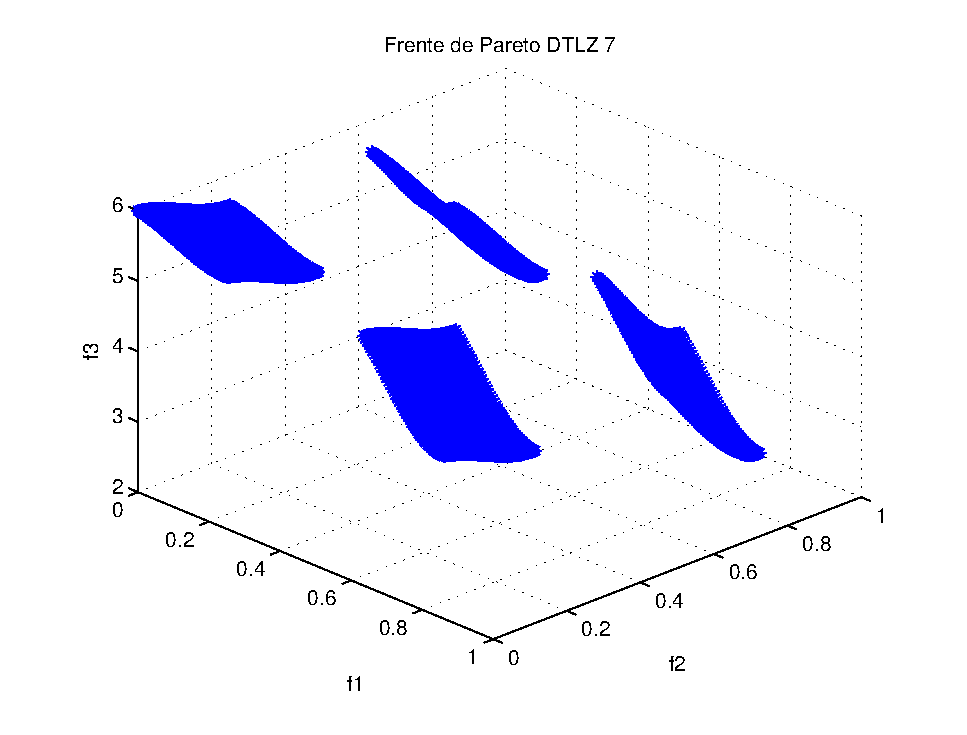
\includegraphics[width=200pt]{Apendices/paretoDTLZ7.eps}
\caption{Frente de Pareto DTLZ7}
\label{fig:DTLZ7}
\end{figure}




\end{chapter}



















